
\section{{\xc EarlyDiscard} Strategy}
\label{sec:earlydiscard}

\begin{figure}
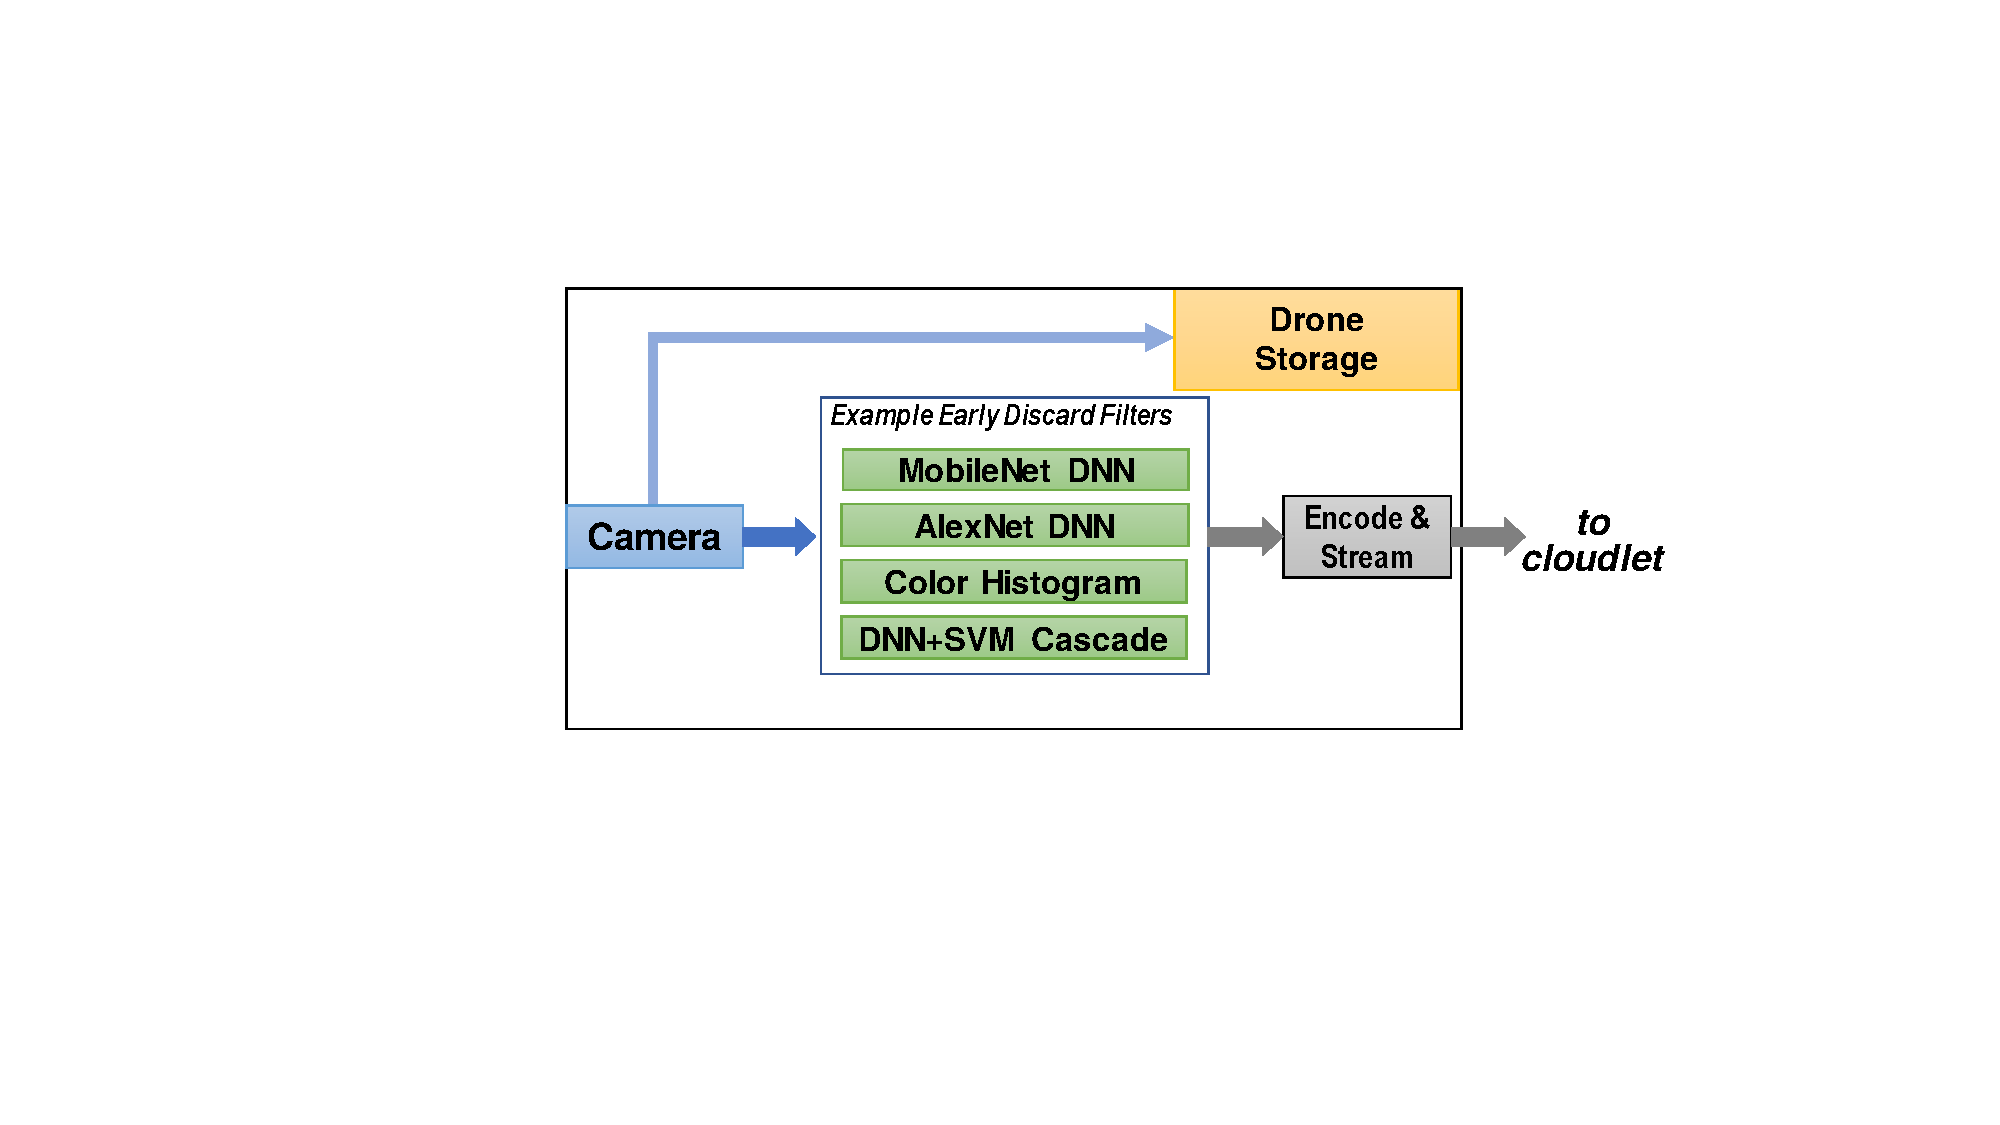
\includegraphics[trim={9cm 6.5cm 5cm 4.8cm},clip,width=\linewidth]{FIGS/fig-ondrone-early-discard.pdf}
\caption{Early Discard on Tier-3 Devices}
\label{fig:ondrone}
\end{figure}


\subsection{Description}
EarlyDiscard is based on the idea of using on-board processing to filter and
transmit only interesting frames in order to save bandwidth when offloading
computation. Frames are considered to be interesting if they capture objects or
events valuable for processing, for instance, survivors for a search task.
Previous work~\cite{Hu2015}~\cite{Naderiparizi2017} leveraged pixel-level
features and multiple sensing modalities to select interesting frames from
hand-held or body-worn cameras. In this section, we explore the use of DNNs to
filter frames from aerial views. The benefits of using DNNs are as follows.
First, DNNs, even shadow ones, are capable of understanding some semantically
meaningful visual information. Their decisions of what to send are based on the
reasoning of image content in addition to pixel-level characteristics. Next,
DNNs are trained and specialized for each task, resulting in their high accuracy
and robustness for that particular task. Finally, compared to a sensor fusing
approach that requires other sensing modalities to be present on Tier-3 devices,
no additional hardware is added to the existing platforms.

Although smartphone-class hardware is incapable of supporting the most accurate
object detection algorithms at full frame rate today, it is typically powerful
enough to support less accurate algorithms.  These {\em weak detectors}, for
instance, MobileNet in Figure~\ref{fig:onboard-dnn-speed}, are typically
designed for mobile platforms or were the state of the art just a few years ago.
In addition, they can be biased towards high recall with only modest loss of
precision. In other words, many clearly irrelevant frames can be discarded by a
weak detector, without unacceptably increasing the number of relevant frames
that are erroneously discarded.  This asymmetry is the basis of the early
discard strategy.

As shown in Figure~\ref{fig:ondrone}, we envision a choice of weak detectors
being available as early discard filters on Tier-3 devices, such as a drone,
with the specific choice of filter being mission-specific.  Based on the
measurements presented in Figure~\ref{fig:onboard-dnn-speed}, we choose cheap
DNNs that can run in real-time as EarlyDiscard filters on Tier-3 devices. Note
that both object detection and image classification algorithms can yield
meaningful early discard results, as it is not necessary to know exactly where
in the frame relevant objects occur --- just an estimate of key object presence
is good enough. This suggests that MobileNet would be a good choice as a weak
detector. For a given image or partial of an image, it can predict whether the
input contains objects of interests. More importantly, MobileNet's speed of 13
ms per frame on the Tier-3 platform Jetson yields more than 75 fps. We therefore
use MobileNet on the drone for early discard in our experiments.

Pre-trained classifiers for MobileNet are available today for objects such as
cars, animals, human faces, human bodies, watercraft, and so on.  However, these
DNN classifiers have typically been trained on images that were captured from a
human perspective --- often by a camera held or worn by a person. These images
typically have the objects at the center of the image and occupy the majority of
the image A drone, however, has an aerial viewpoint and objects look rather
different.  To improve classification accuracy on drones, we used {\em transfer
learning}~\cite{Yosinski2014} to finetune the pre-trained classifiers on small
training sets of images that were captured from an aerial viewpoint. Finetuning
not only allows us to adapt pre-trained classifiers to drone views, but also
makes it possible to target custom objects of interests that are not in the
original dataset, for instance, survivors in orange life jacket. The process of
fine-tuning involves initial re-training of the last DNN layer, followed by
re-training of the entire network until convergence. Transfer learning enables
accuracy to be improved significantly for aerial images without incurring the
full cost of creating a large training set captured from an aerial viewpoint.

\begin{figure}
\centering
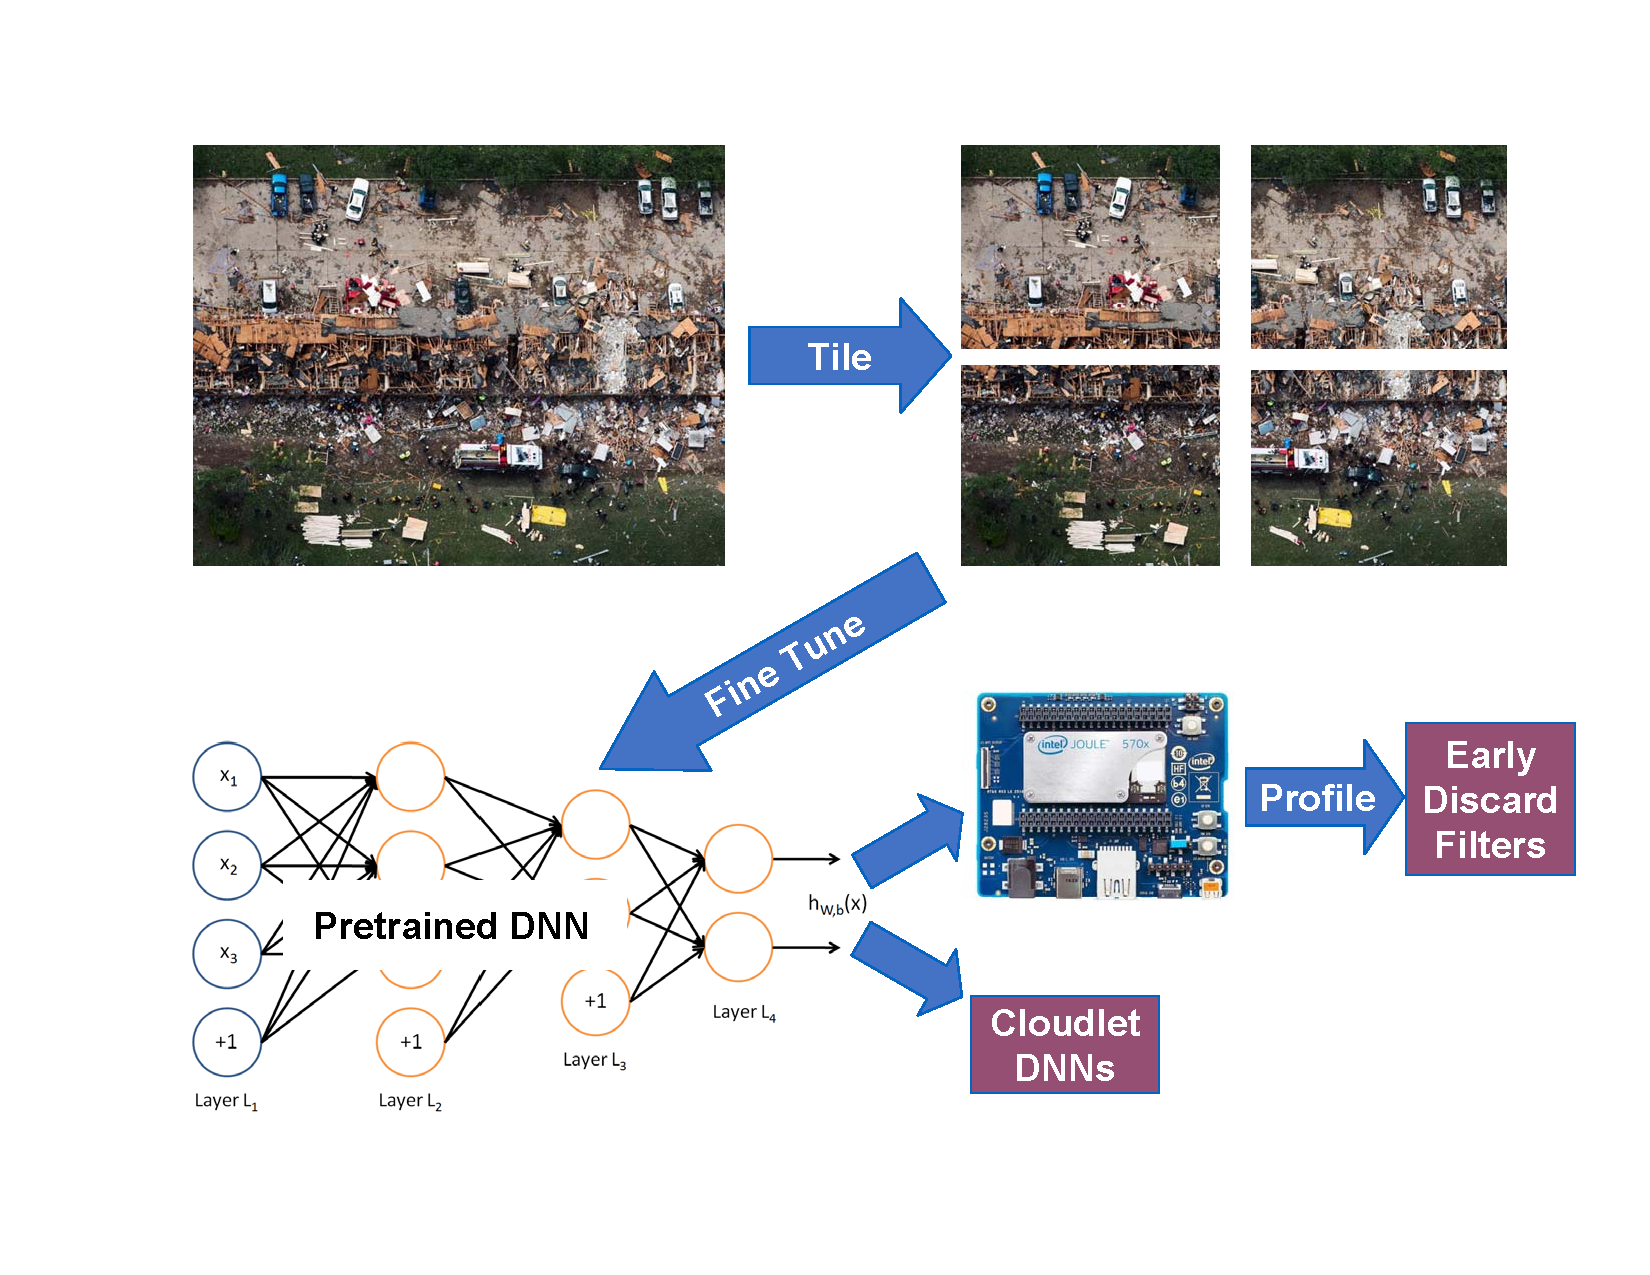
\includegraphics[width=0.8\linewidth]{FIGS/fig-training.pdf}
\caption{Tiling and DNN Fine Tuning}
\label{fig:tiling}
\end{figure}

Drone images are typically captured from a significant height, and hence objects
in such an image are small.  This interacts negatively with the design of many
DNNs, which first transform an input image to a fixed low resolution --- for
example, 224x224 pixels in MobileNet. Many important but small objects in the
original image become less recognizable.  It has been shown that small object
size correlates with poor accuracy in DNNs~\cite{Huang2017}.  To address this
problem, we {\em tile} high resolution frames into multiple sub-frames and then
perform recognition on the sub-frames as a batch.  This is done offline for
training, as shown in Figure~\ref{fig:tiling}, and also for online inference on
the drone and on the cloudlet.  The lowering of resolution of a sub-frame by a
DNN is less harmful, since the scaling factor is smaller.  Objects are
represented by many more pixels in a transformed sub-frame than if the entire
frame had been transformed.  The price paid for tiling is increased
computational demand.  For example, tiling a frame into four sub-frames results
in four times the classification workload. Note that this increase in workload
typically does not translates into the same increase in inference time, as
workloads can be batched together to leverage hardware parallelism for a reduced
total inference time.

\begin{figure}
\centering
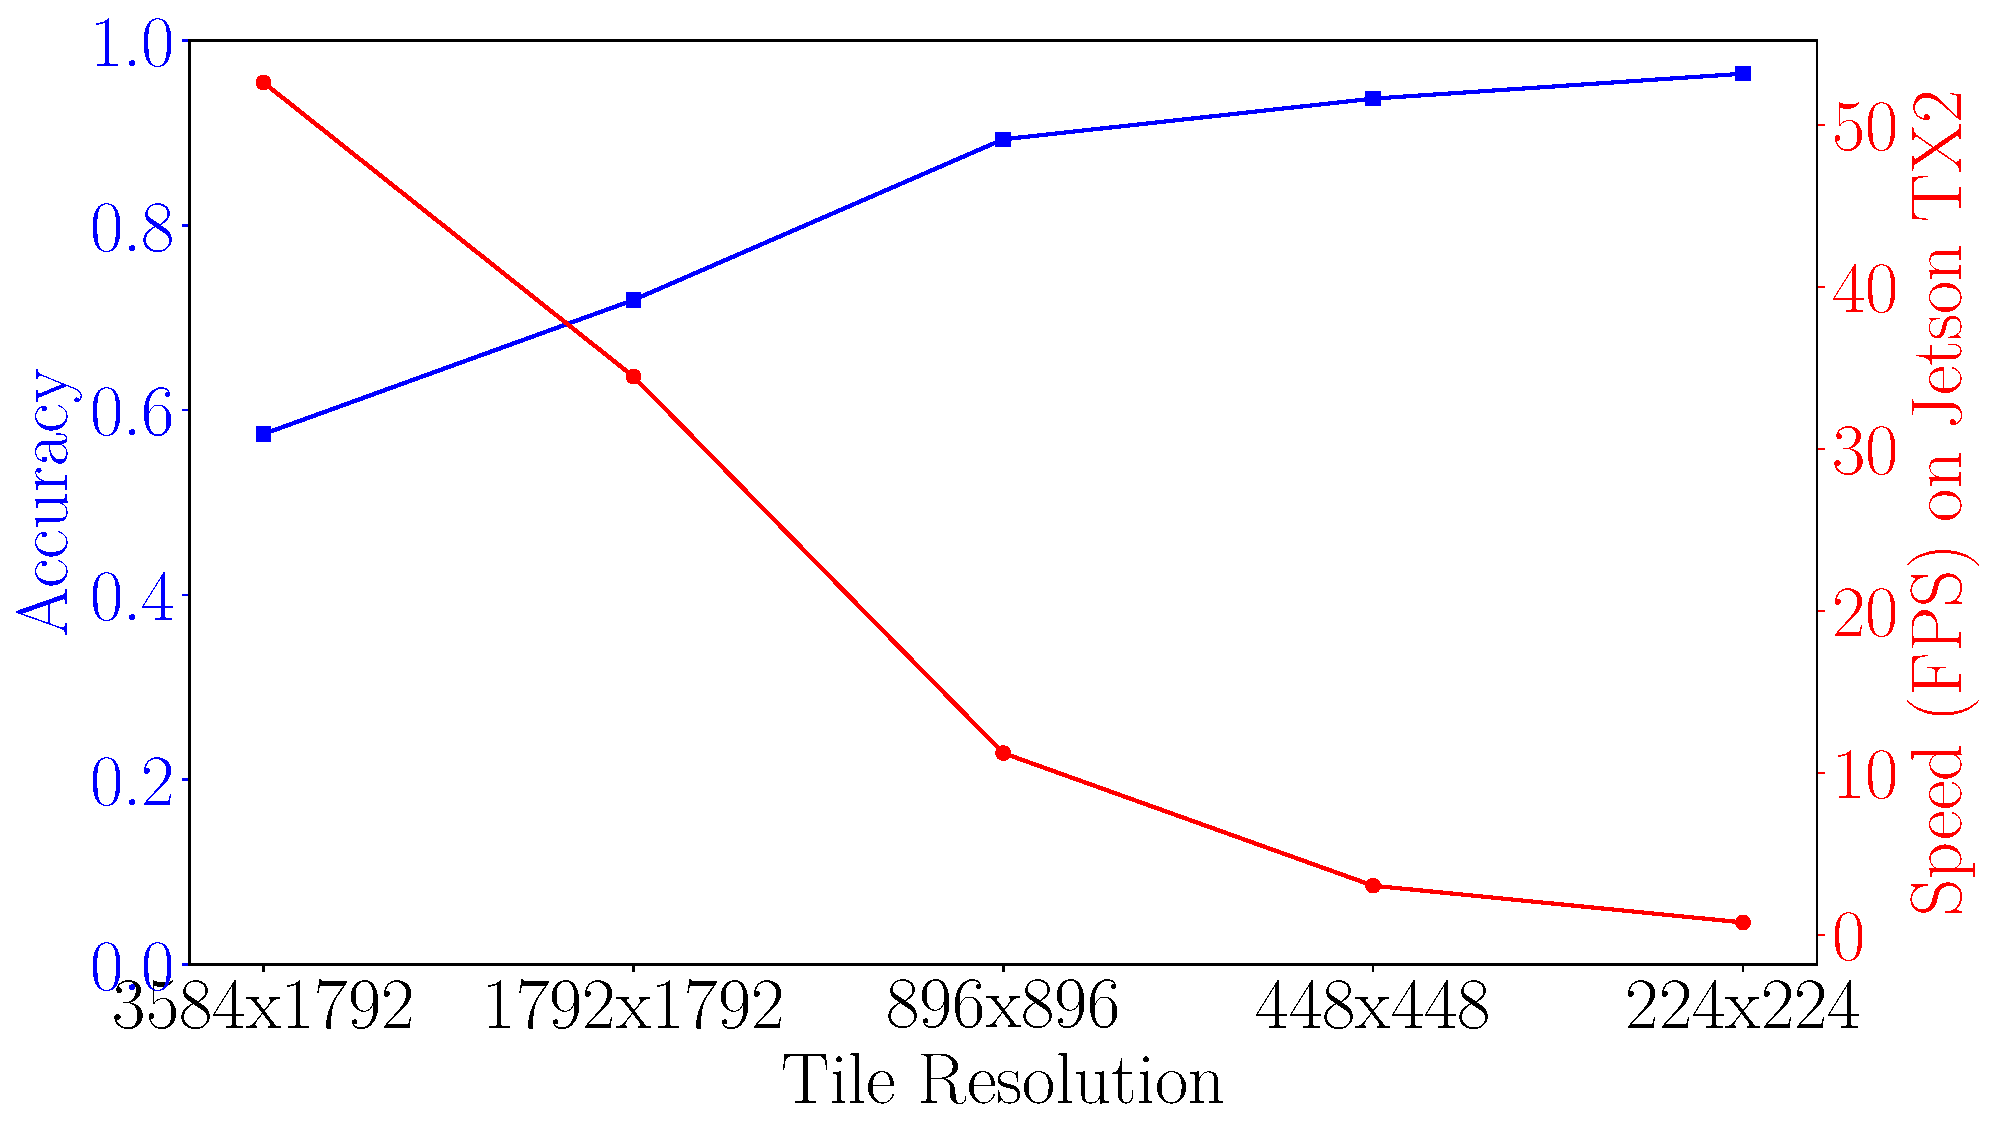
\includegraphics[width=.8\linewidth]{FIGS/fig-tile-resolution-speed-accuracy.pdf}
\caption{Speed-Accuracy Trade-off of Tiling}
\label{fig:earlydiscard-tile-accuracy-speed}
\end{figure}


\subsection{Experimental Setup}

Our experiments on the {\xc EarlyDiscard} strategy used the same benchmark suite
described in Section~\ref{sec:dumbdrone-setup}. We used Jetson TX2 as the Tier-3
device platform. We run MobileNet filters to get predictions on whether
sub-frames contain objects of interests. We compare the predictions with ground
truths (e.g. whether a sub-frame is indeed interesting) to evaluate the
effectiveness of EarlyDiscard. Both frame-based and event-based metrics are used
in the evaluation.

\begin{figure}
\centering
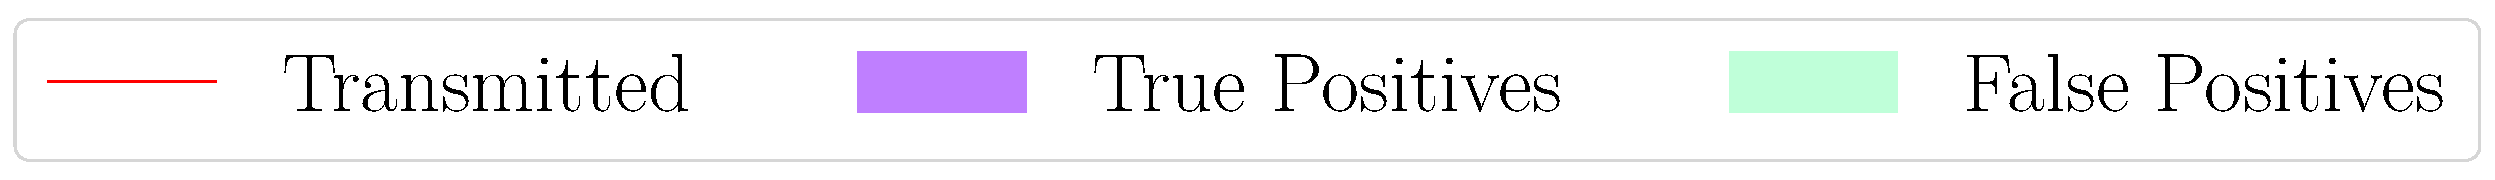
\includegraphics[width=\linewidth]{FIGS/fig-event-recall-frame-percentage-legend.pdf}\\
    \vspace{.5in}
\begin{minipage}[]{0.45\linewidth}
\centering
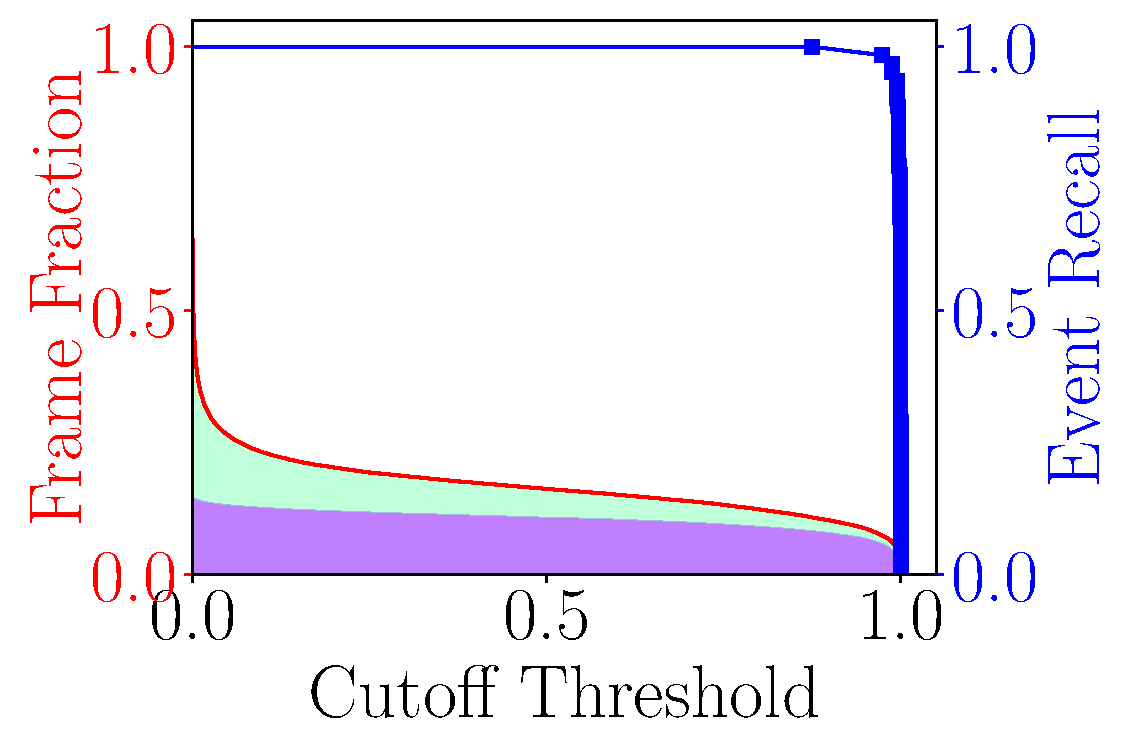
\includegraphics[width=\linewidth]{FIGS/fig-event-recall-frame-percentage-vs-threshold-okutama.pdf}\\
{(a) T1}
\end{minipage}
\begin{minipage}[]{0.45\linewidth}
\centering
    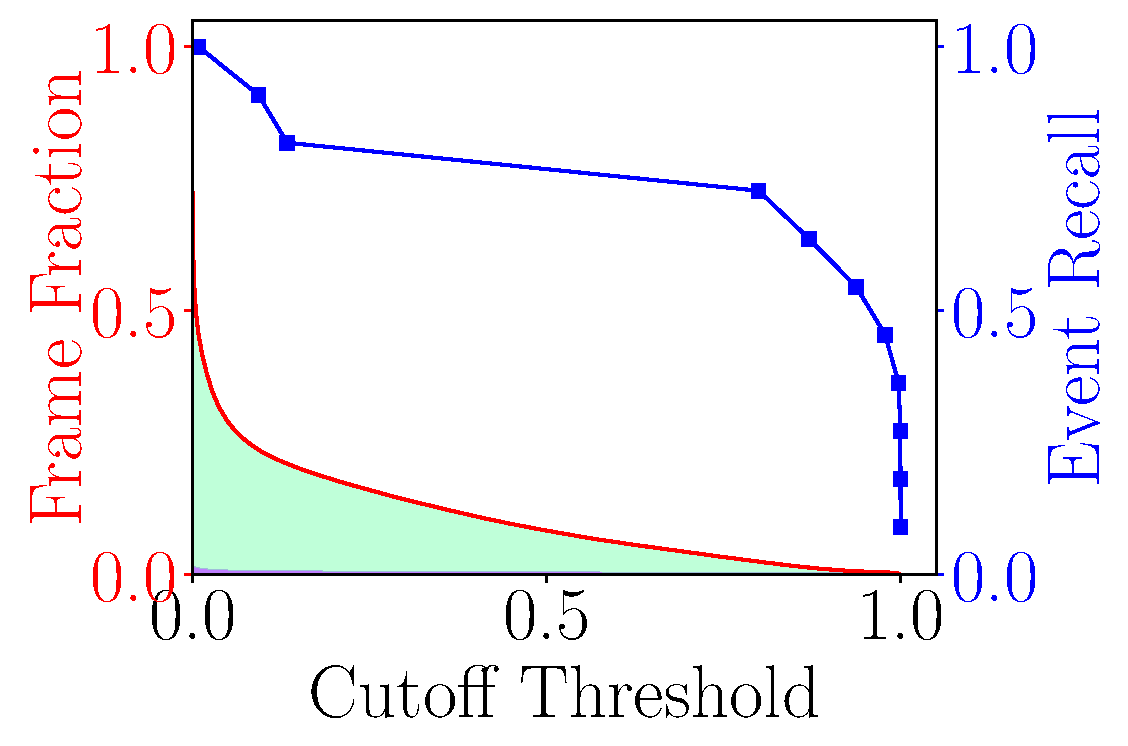
\includegraphics[width=\linewidth]{FIGS/fig-event-recall-frame-percentage-vs-threshold-stanford.pdf}\\
{(b) T2}
\end{minipage}

\vspace{.5in}

\begin{minipage}[]{0.45\linewidth}
\centering
    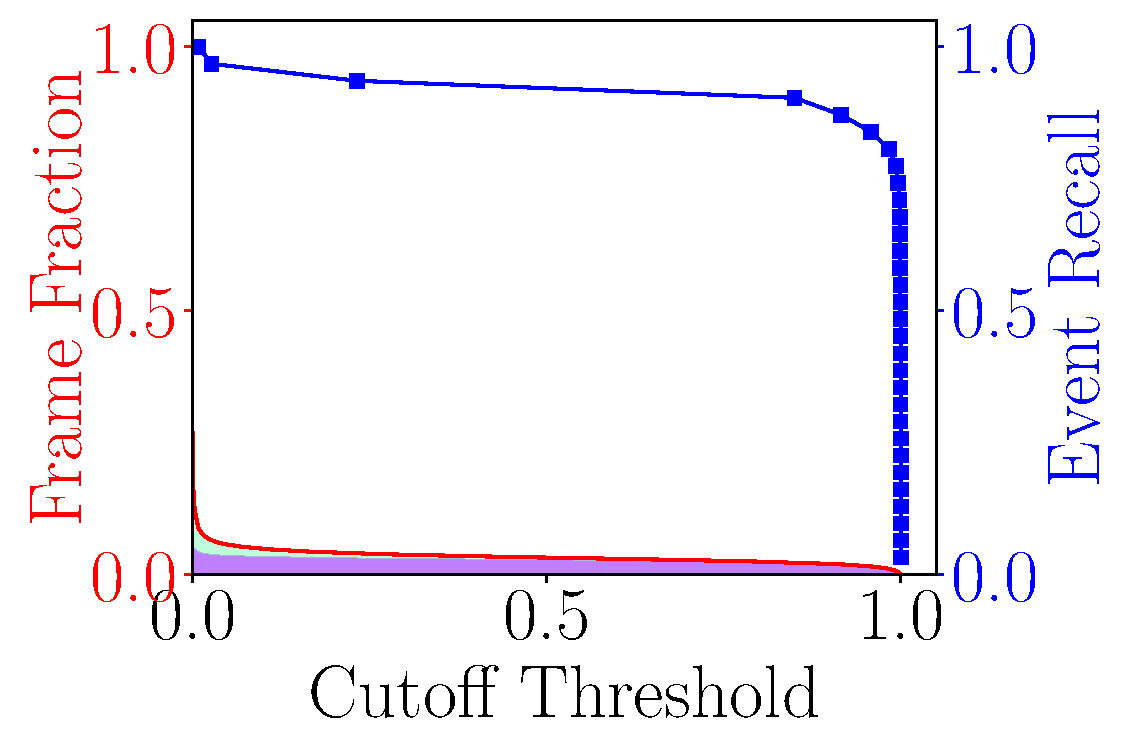
\includegraphics[width=\linewidth]{FIGS/fig-event-recall-frame-percentage-vs-threshold-raft.pdf}\\
{(c) T3}
\end{minipage}
\begin{minipage}[]{0.45\linewidth}
\centering
    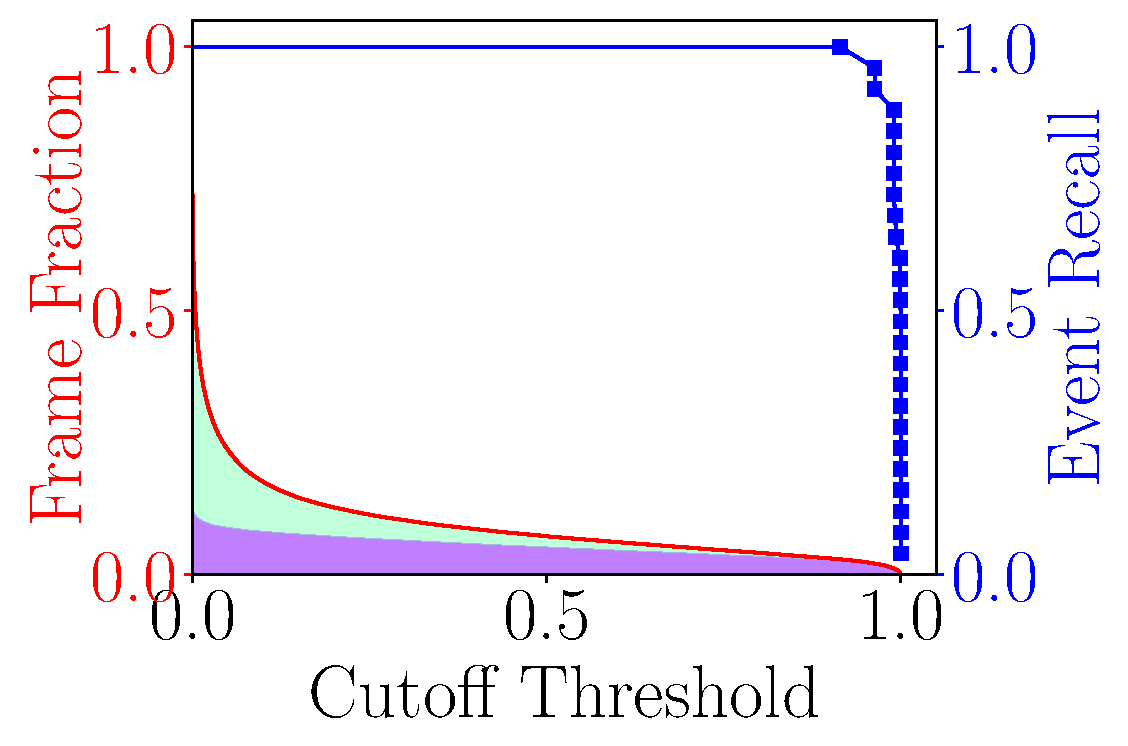
\includegraphics[width=\linewidth]{FIGS/fig-event-recall-frame-percentage-vs-threshold-elephant.pdf}\\
{(c) T4}
\end{minipage}

    \vspace{.5in}
\caption{Bandwidth Breakdown}
\label{fig:earlydiscard-frame-percent-breakdown}
\end{figure}

\subsection{Results of Early Discard Filters}
\label{sec:earlydiscard-result}

EarlyDiscard is able to significantly reduce the bandwidth consumed while
maintaining high result accuracy and low average delay. For three out of four
tasks, the average bandwidth is reduced by a factor of ten. Below we present
our results in detail.

\subsubsection{Effects of Tiling}
% \noindent{\textbf{Effects of Tiling}}: 
Tiling is used to improve the accuracy
for high resolution aerial images. We used the Okutama Action Dataset, whose
attributes are shown in row T1 of Figure~\ref{fig:benchmarksuite}, to explore
the effects of tiling.  For this dataset,
Figure~\ref{fig:earlydiscard-tile-accuracy-speed} shows how speed and accuracy
change with tile size.  Accuracy improves as tiles become smaller, but the
sustainable frame rate drops.  We group all tiles from the same frame in a
single batch to leverage parallelism, so the processing does not change linearly
with the number of tiles. The choice of an operating point will need to strike a
balance between the speed and accuracy.  In the rest of the chapter, we use two
tiles per frame by default. 

\subsubsection{Drone Filter Accuracy}
% \noindent{\textbf{Drone Filter Accuracy}}: 
The output of a drone filter is the
probability of the current tile being ``interesting.''  A tunable {\em cutoff
threshold} parameter specifies the threshold for transmission to the cloudlet.
All tiles, whether deemed interesting or not, are still stored in the drone
storage for offline processing.

Since objects have temporal locality in videos, we define an event (of an
object) in a video to be consecutive frames containing the same object of
interests. For example, the appearance of the same red raft in T3 in consecutive
45 frames constitutes a single event. A correct detection of an event is defined
as at least one of the consecutive frames being transmitted to the cloudlet.  

Figure~\ref{fig:earlydiscard-frame-percent-breakdown} shows our results on all
four tasks. Blue lines in Figure~\ref{fig:earlydiscard-frame-percent-breakdown}
shows how the event recalls of drone filters for different tasks change as a
function of cutoff threshold. The MobileNet DNN filter we used is able to detect
all the events for T1 and T4 even at a high cutoff threshold. For T2 and T3, the
majority of the events are detected. Achieving high recall on T2 and T3 (on the
order of 0.95 or better) requires setting a low cutoff threshold.  This leads to
the possibility that many of the transmitted frames are actually uninteresting
(i.e., false positives).

\subsubsection{False negatives}
As discussed earlier, false negatives are
a source of concern with early discard.  Once the drone drops a frame
containing an important event, improved cloudlet processing cannot help. The
results in the third column of Figure~\ref{fig:early-discard-results} confirm
that there are no false negatives for T1 and T4 at a cutoff threshold of 0.5.
For T2 and T3, lower cutoff thresholds are needed to achieve perfect recalls.

\subsubsection{Result latency}
The contribution of early discard processing to total result latency
is calculated as the average time difference between the first frame
in which an object occurs (i.e., first occurrence in ground truth) and
the first frame containing the object that is transmitted to the
backend (i.e., first detection).  The results in the fourth column of
Figure~\ref{fig:early-discard-results} confirm that early discard
contributes little to result latency.  The amounts range from 0.1~s
for T1 to 12.7~s for T3.  At the timescale of human actions
such as dispatching of a rescue team, these are negligible delays.

\begin{figure}
\centering
\begin{tabular}{|c|c|c|c|c|c|c|}
\hline
   &Task Total Events   &Detected Events       &Avg Delay & Total Data &Avg B/W &Peak B/W\\
   & & &(s)&(MB)&(Mbps)&(Mbps)\\ 

\hline
T1 & \phantom{0}62  & 100~\%       &  \phantom{0}0.1&\phantom{0}441  &  5.10     &   10.7  \\
\hline
T2 & \phantom{0}11  & \phantom{0}73~\%      & \phantom{0}4.9 & \phantom{00}13            &  0.03 & \phantom{0}7.0 \\ % 100% recall at 47% of frames, 82% recall at 21% of frames
\hline
T3 & \phantom{0}31  & \phantom{0}90~\%  & 12.7 & \phantom{00}93  &  0.24 &  \phantom{0}7.0 \\ % 100% recall at 9% frames
\hline
T4 & \phantom{0}25  & 100~\%       & \phantom{0}0.3 & \phantom{0}167  &  0.43 &  \phantom{0}7.0 \\
\hline
\end{tabular}\\
\caption{Recall, Event Latency and Bandwidth at Cutoff Threshold 0.5}
\label{fig:early-discard-results}
\end{figure}


\subsubsection{Bandwidth}
Columns 5--7 of Figure~\ref{fig:early-discard-results} pertain to wireless
bandwidth demand for the benchmark suite with early discard.  The figures shown
are based on H.264 encoding of each individual frames in the drone-cloudlet
video transmission. Average bandwidth is calculated as the total data
transmitted divided by mission duration.  Comparing column 5 of
Figure~\ref{fig:early-discard-results} with column 2 of
Figure~\ref{fig:baseline}, we see that all videos in the benchmark suite are
benefited by early discard (Note T3 and T4 have the same test dataset as T2).
For T2, T3, and T4, the bandwidth is reduced by more than 10x. The amount of
benefit is greatest for rare events (T2 and T3).  When events are rare, the
drone can drop many frames.

Figure~\ref{fig:earlydiscard-frame-percent-breakdown} provides deeper insight
into the effectiveness of cutoff-threshold on event recall. It also shows how
many true positives (violet) and false positives (aqua) are
transmitted. Ideally, the aqua section should be zero.  However for T2, most
frames transmitted are false positives, indicating the early discard filter has
low precision.  The other tasks exhibit far fewer false positives.  This
suggests that the opportunity exists for significant bandwidth savings if
precision could be further improved, without hurting recall.

\subsection{Use of Sampling}

\begin{figure}[h]
    \centering
    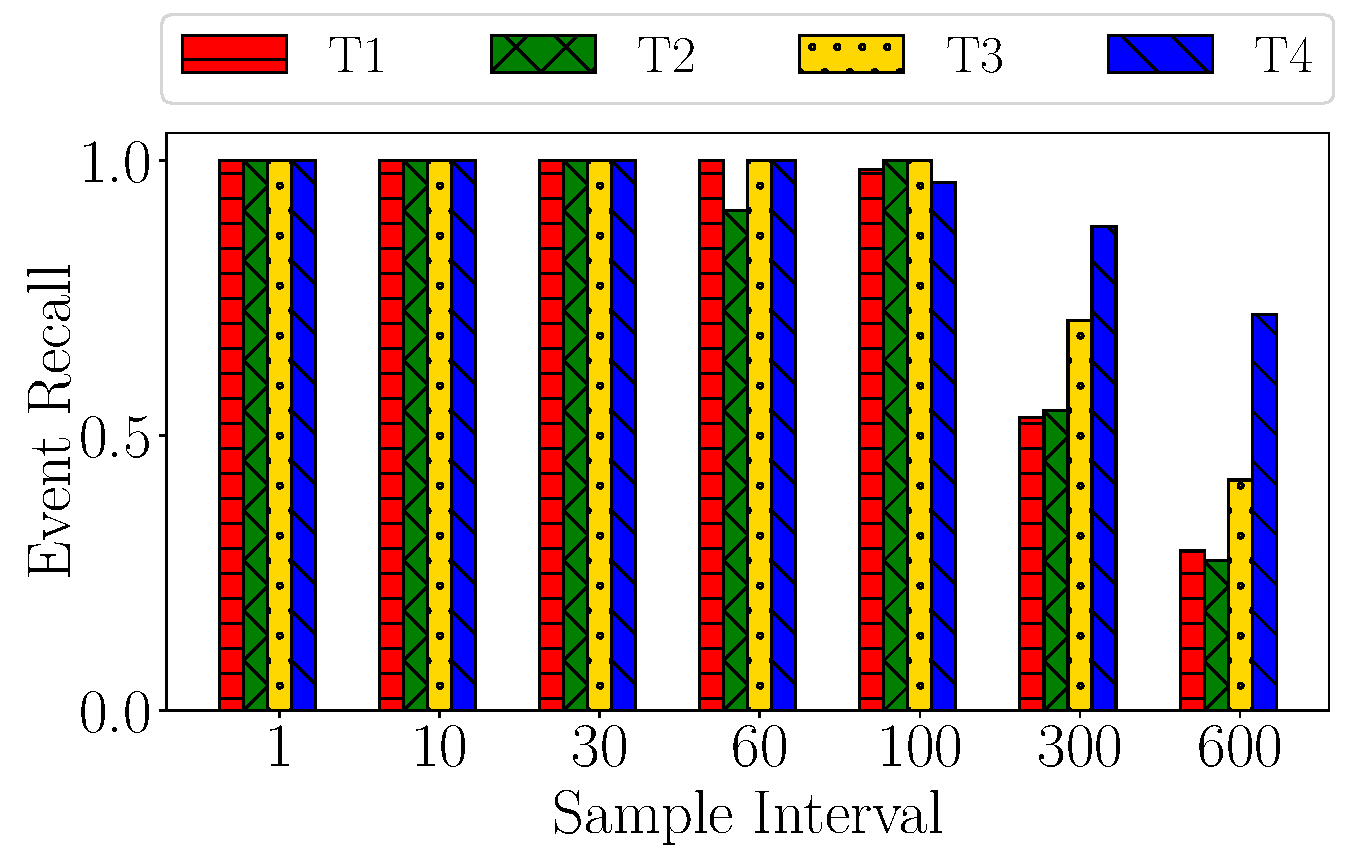
\includegraphics[width=.9\linewidth]{FIGS/fig-random-select-interval-recall-hatch.pdf}
\caption{Event Recall at Different Sampling Intervals}
\label{fig:sampling-only}
\end{figure}


\begin{figure}[h]
\centering
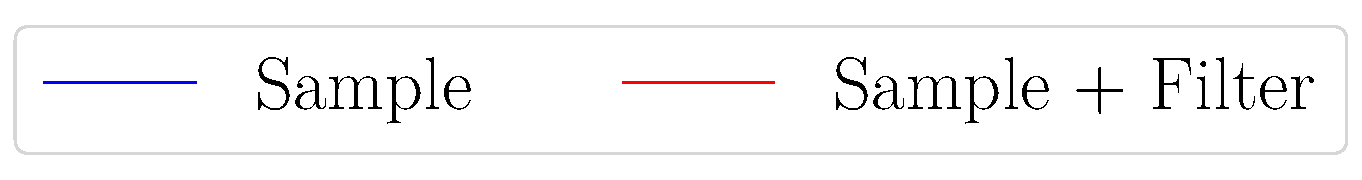
\includegraphics[width=0.7\linewidth]{FIGS/fig-recall-frame-aggregated-legend.pdf}

\begin{minipage}[]{0.47\linewidth}
\centering
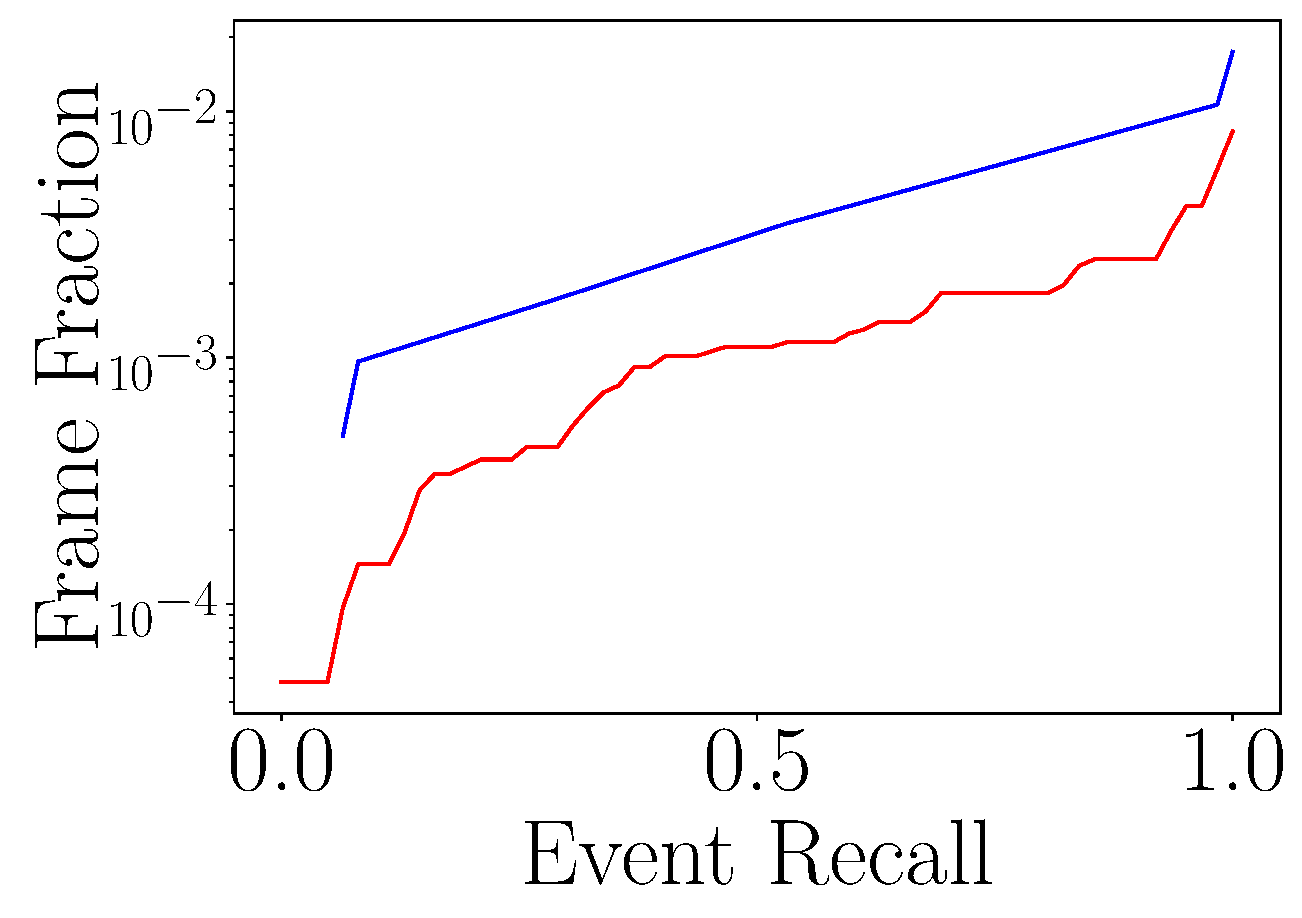
\includegraphics[trim={0.5cm 0.5cm 0 0},clip,width=\linewidth]{FIGS/fig-random-select-and-filter-recall-frame-okutama-aggregated.pdf}\\
{(a) T1}
\end{minipage}
\begin{minipage}[]{0.47\linewidth}
\centering
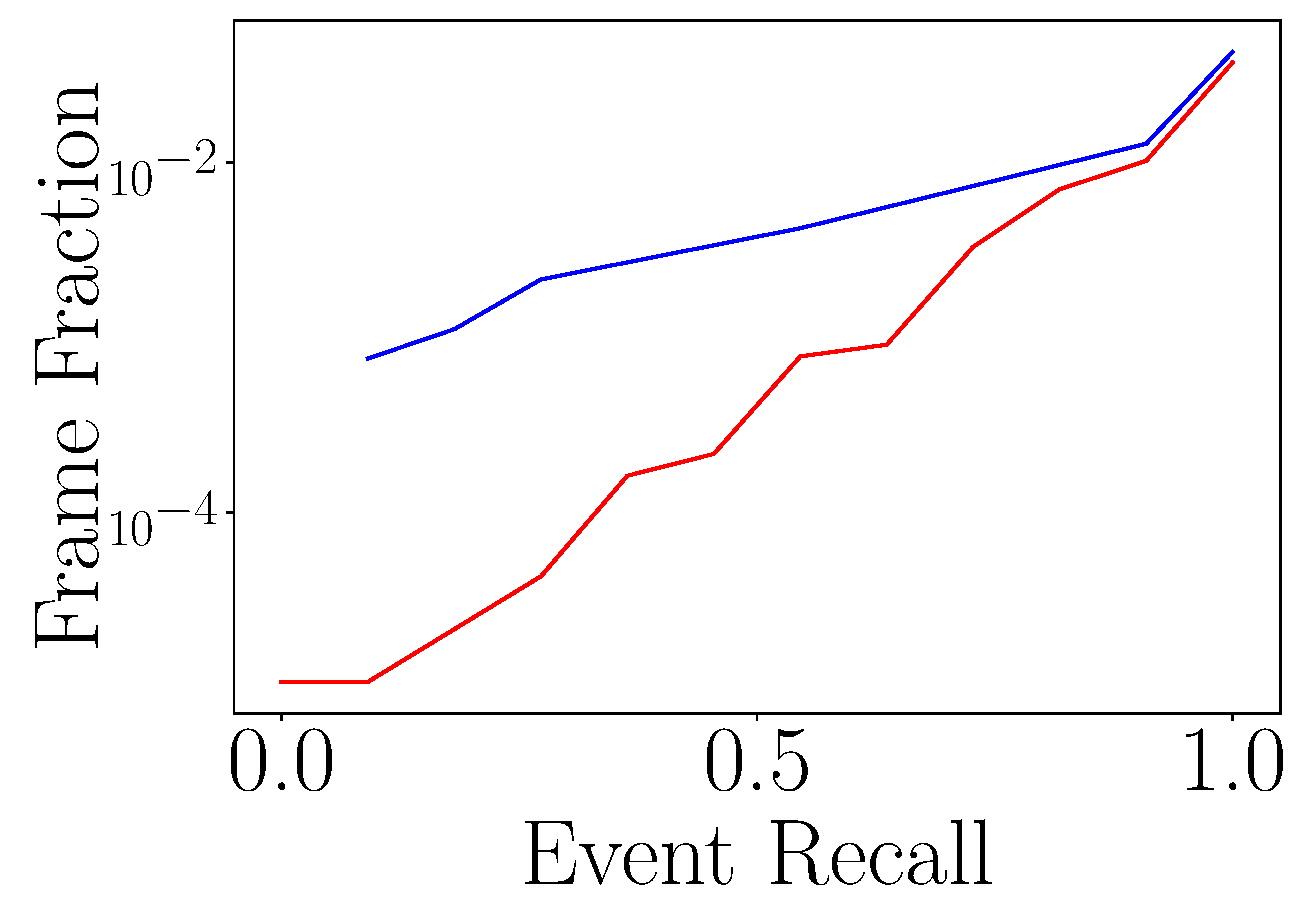
\includegraphics[trim={0.5cm 0.5cm 0 0},clip,width=\linewidth]{FIGS/fig-random-select-and-filter-recall-frame-stanford-aggregated.pdf}
{(b) T2}
\end{minipage}
\begin{minipage}[]{0.47\linewidth}
\centering
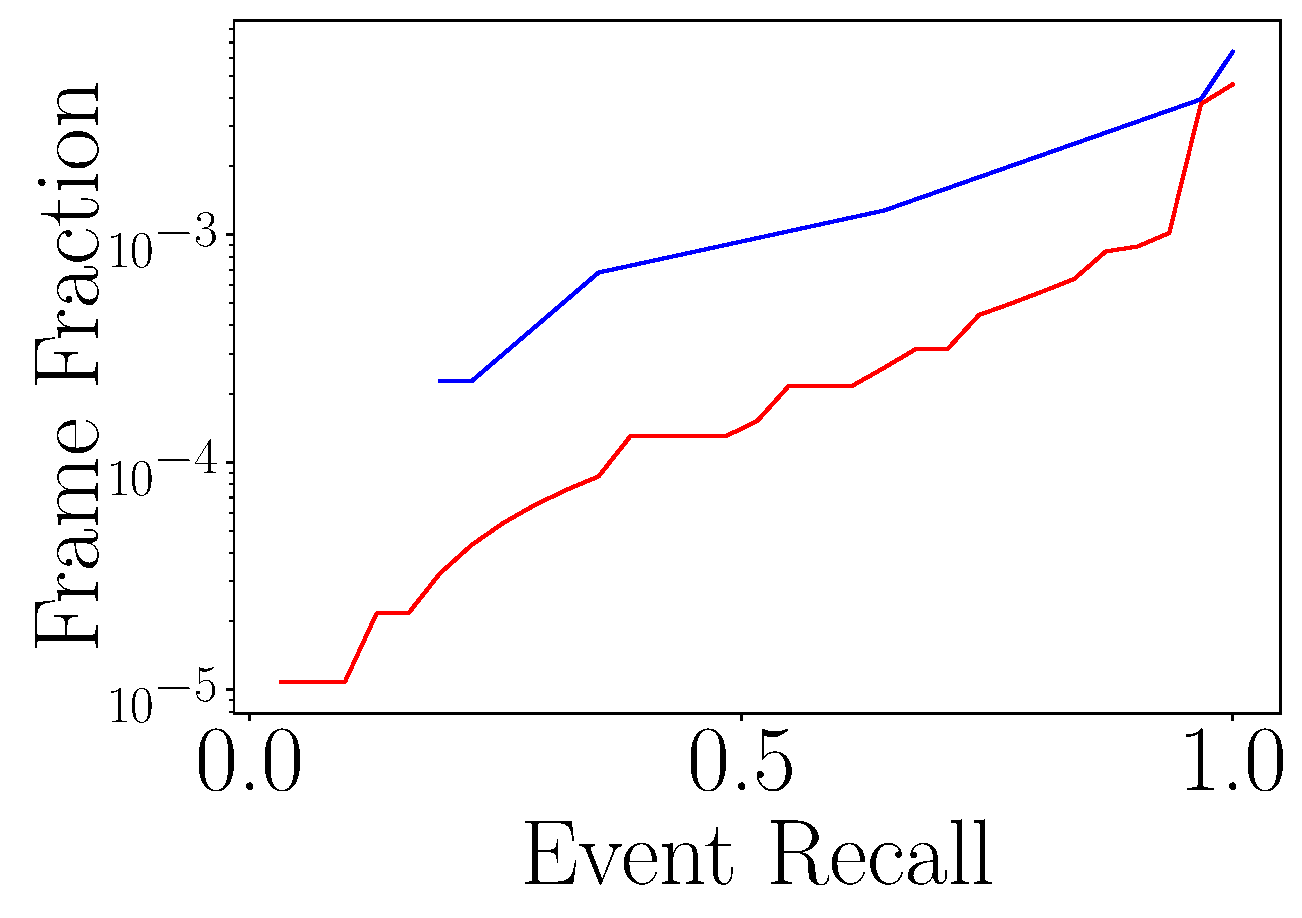
\includegraphics[trim={0.5cm 0.5cm 0 0},clip,width=\linewidth]{FIGS/fig-random-select-and-filter-recall-frame-raft-aggregated.pdf}
{(c) T3}
\end{minipage}
\begin{minipage}[]{0.47\linewidth}
\centering
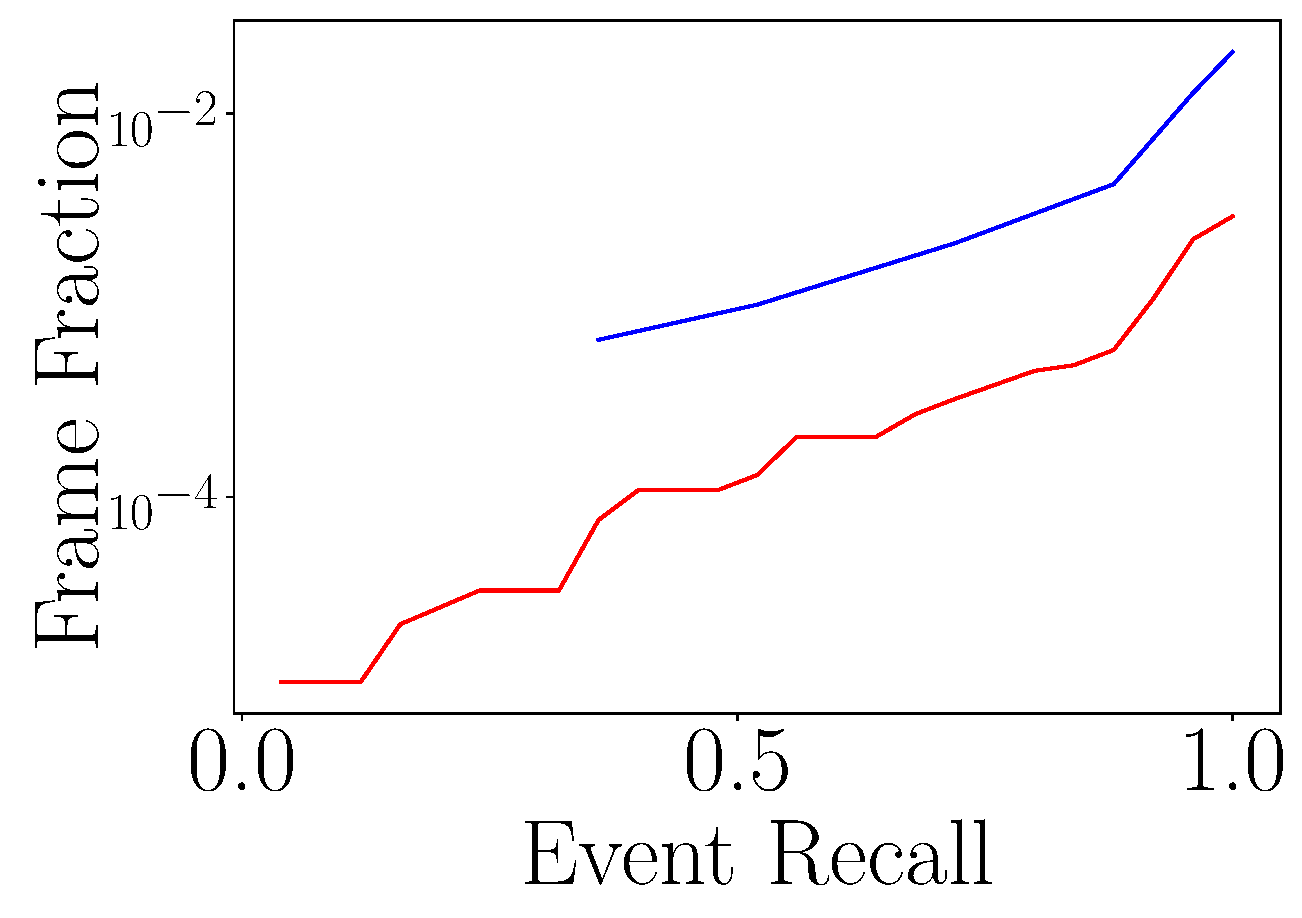
\includegraphics[trim={0.5cm 0.5cm 0 0},clip,width=\linewidth]{FIGS/fig-random-select-and-filter-recall-frame-elephant-aggregated.pdf}
{(c) T4}
\end{minipage}
\caption{Sample with Early Discard. Note the log scale on y-axis.}
\label{fig:sampling-discard}
\end{figure}

\begin{figure}[h]
\centering
\begin{tabular}{|c|c|c|c|c|}
\hline
JPEG Frame Sequence  & H264 High Quality  & H264 Medium Quality & H264 Low Quality \\
(MB) & (MB) & (MB) & (MB)\\
\hline
5823 & 3549  & 1833 & 147\\
\hline
\end{tabular}\\
\vspace{0.1in}
\begin{captiontext}
H264 high quality uses Constant Rate Factor (CRF) 23. Medium
uses CRF 28 and low uses 40~\cite{Merritt2007}.
\end{captiontext}
\caption{Test Dataset Size With Different Encoding Settings}
\label{fig:video-vs-images}
\end{figure}

Given the relatively low precision of the weak detectors, a significant number 
of false positives are transmitted.  Furthermore, the occurrence of an object will
likely last through many frames, so true positives are also often redundant for 
simple detection tasks.  Both of these result in excessive
consumption of precious bandwidth.  
This suggests that simply restricting the number of transmitted
frames by sampling may help reduce bandwidth consumption.  

Figure~\ref{fig:sampling-only} shows the effects of 
sending a sample of frames from the drone, without any
content-based filtering.  Based on these results, we can reduce
the frames sent as little as one per second and still get
adequate recall at the cloudlet.  Note that this result is very
sensitive to the actual duration of the events in the videos.
For the detection tasks outlined here, most of the events (e.g.,
presences of a particular elephant) last for many seconds (100's
of frames), so such sparse sampling does not hurt recall.
However, if the events were of short duration, e.g., just a few
frames long, then this method would be less effective, as
sampling may lead to many missed events (false negatives).  

Can we use content-based filtering along with sampling to further
reduce bandwidth consumption?  Figure~\ref{fig:sampling-discard}
shows results when running early discard on a sample of the
frames. This shows that for the same recall, we can reduce the
bandwidth consumed by another factor of 5 on average over sampling alone.
This effective combination can reduce the average bandwidth
consumed for our test videos to just a few hundred kilobits
per second.  Furthermore, more processing time is available per
processed frame, allowing more sophisticated algorithms to be
employed, or to allow smaller tiles to be used, improving
accuracy of early discard.  

One case where sampling is not an effective solution is when all frames
containing an object need to be sent to the cloudlet for some form of activity
or behavior analysis from a complete video sequence.  In this case, bandwidth
will not reduce much, as all frames in the event sequence must be sent.
However, the processing time benefits of sampling may still be exploited,
provided all frames in a sample interval are transmitted on a match.  


\subsection{Effects of Video Encoding}

One advantage of the {\xc Dumb} strategy is that since all
frames are transmitted, one can use a modern video encoding to
reduce transmission bandwidth.  With early discard, only a subset
of disparate frames are sent.  These will likely need to be
individually compressed images, rather than a video stream.  How
much does the switch from video to individual frames affect
bandwidth?  

In theory, this can be a significant impact. Video encoders leverage the
similarity between consecutive frames, and model motion to efficiently encode
the information across a set of frames. Image compression can only exploit
similarity within a frame, and cannot efficiently reduce number of bits needed
to encode redundant content across frames. To evaluate this difference, we start
with extracted JPEG frame sequences of our video data set. We encode the frame
sequence with different H.264 settings. Figure~\ref{fig:video-vs-images}
compares the size of frame sequences in JPEG and the encoded video file sizes.
We see only about 3x difference in the data size for the medium quality. We can
increase the compression (at the expense of quality) very easily, and are able
to reduce the video data rate by another order of magnitude before quality
degrades catastrophically.

However, this compression does affect analytics. Even at medium quality level,
visible compression artifacts, blurring, and motion distortions begin to appear.
Initial experiments analyzing compressed videos show that these distortions do
have a negative impact on accuracy of analytics. Using average precision
analysis, a standard method to evaluate accuracy, we see that the 
most accurate model (Faster-RCNN ResNet101) on low quality videos performs similarly
to the less accurate model (Faster-RCNN InceptionV2) on high quality
JPEG images. This negates the benefits of using the state-of-art models.

In our EarlyDiscard design, we pay a penalty of sending frames instead of a
compressed low quality video stream. This overhead (approximately 30x) is
compensated by the 100x reduction in frames transmitted due to sampling with
early discard. In addition, the selective frame transmission preserves the
accuracy of the state-of-art detection techniques.

Finally, one other option is to treat the set of disparate frames as a sequence
and employ video encoding at high quality. This can ultimately eliminate the per
frame overhead while maintaining accuracy. However, this will require a complex setup with
both low-latency encoders and decoders, which can generate output data
corresponding to a frame as soon as input data is ingested, with no buffering,
and can wait arbitrarily long for additional frame data to arrive. 

For the experiments in the rest of this chapter, we only account for the
fraction of frames transmitted, rather than the choice of specific encoding
methods used for those frames.



%-------------- LEAVE THIS AT THE END OF THIS FILE --------------------
\begin{comment}
% Satya: Save this old table because it has lots of details that 
% are not included in the smaller table that is in the paper
\begin{figure*}[]
\centering
\begin{tabular}{|p{2cm}|p{2cm}|p{2cm}|p{3cm}|p{3cm}|p{3cm}|}
\hline
Task                     & Task Description                                                                           & Dataset                & Dataset Description                                                                                                                & Train Videos                                                                                     & Test Videos                                                         \\ \hline
Human Detection 	& Detect human beings in daily life scene. Report any humans detected.			& 	UCF Aerial Action Dataset \href{http://crcv.ucf.edu/data/UCF_Aerial_Action.php}{link}				& A video dataset for aerial view of human actions. 4 videos, 107184 frames in total. 720x480 @ 30FPS. 			&  Select 2 videos with drone moving.  57430 frames.			& Select 2 videos with drone moving. 49754 frames.\\ \hline
Human Detection          & Detect human beings in a search and rescue scene. Report any humans detected.              & Okutama Action Dataset~\cite{Barekatain2017} 	& A video dataset for aerial view concurrent human action detection.  33 videos, 59842 frames in total. 3840x2160 @ 30FPS.           & Select 9 videos in which drones are actively moving, similar to search and rescue. 17763 frames. & Randomly select 3 videos in which drones are moving.  6014 frames.  \\ \hline
Human Activity Detection & Detect human activities such as waving hands                                               & Okutama Action Dataset & Same as above                                                                                                                      & Same as above                                                                                    & Same as above                                                       \\ \hline
Moving Car Detection     & Detect cars in a search and rescue scene that are moving. Report any moving cars detected. & Stanford Drone Dataset~\cite{Robicquet2016} & An aerial video dataset of cars and people navigating in a university campus. 60 videos, 522497 frames in total. $\sim$HD @ 30FPS. & Select 16 videos in which exists moving cars. 179992 frames.                                     & Randomly select 5 videos in which exists moving cars. 60249 frames. \\ \hline
Raft Detection           & Detect raft in a flooding scene                               & Collected 11 Youtube Videos \href{https://www.dropbox.com/sh/zksp1pzc1ix5hlw/AAB3HEhx-yLAJVR1Q3HnFpsWa?dl=0}{[Links]}       & Aerial-view videos with rafts. 11 videos. 54395 frames in total. $\sim$720P @ 30 FPS.                                                                                                    & 8 videos of rafting as training set. 43017 frames.                                      &  3 videos that resemble search and rescue scenarios. 11378 frames.                                               \\ \hline
Animal Detection         & Detect elephants in their natural habitat                     & Collected 11 Youtube Videos \href{https://www.dropbox.com/sh/3uly2qqwbzjasaa/AABiWSzPD_5uzmvCy3meqPKma?dl=0}{[Links]}      &  Aerial-view videos containing elephants in their natural habitat. 11 videos. 54203 frames in total. $\sim$720P @ 30FPS.                                                                         & Randomly selected 8 videos as training set. 39466 frames.                      & Randomly selected 3 videos as test set. 14737 frames.                \\ \hline
\end{tabular}
\caption{Task and Dataset}
\label{fig:task-and-dataset}
\end{figure*}
\end{comment}

